% =====================================================================
%  RFC -- secao "Fluxos" (Implementacao)
%  Arquivo compilavel sozinho para revisao. Para levar para a RFC,
%  copie o trecho entre "INICIO DA SECAO" e "FIM DA SECAO".
%  Pacotes necessarios na RFC: amssymb, enumitem, tikz (arrows.meta), url, underscore
% =====================================================================
\documentclass[11pt,a4paper]{article}

\usepackage[a4paper,margin=2.2cm]{geometry}
\usepackage[utf8]{inputenc}
\usepackage[T1]{fontenc}
\IfFileExists{lmodern.sty}{\usepackage{lmodern}}{\usepackage{mathptmx}\usepackage{courier}}
\IfFileExists{portuguese.ldf}{\usepackage[brazil]{babel}}{}
\usepackage{microtype}
\usepackage{amsmath,amssymb}
\usepackage{enumitem}
\usepackage{tikz}
\usetikzlibrary{arrows.meta}
\usepackage[hidelinks]{hyperref}
\usepackage{url}
\usepackage[strings]{underscore}

\newcommand{\tb}[1]{\texttt{#1}}
\newcommand{\rs}{R\$\,}
\setlength{\parindent}{0pt}
\setlength{\parskip}{3pt}
\emergencystretch=3em
\setlist[enumerate]{itemsep=1pt,topsep=2pt,leftmargin=1.6em}
\setlist[itemize]{itemsep=1pt,topsep=2pt,leftmargin=1.4em}

\begin{document}

% ======================= INICIO DA SECAO =============================
\subsection*{Fluxos}

\textbf{Esqueleto comum.} Toda operação que move dinheiro segue a mesma ordem:
\emph{ler $\to$ travar $\to$ checar idempotência $\to$ decidir $\to$ escrever $\to$ \tb{commit}}.
Nenhuma escrita acontece antes da última verificação, então uma recusa não tem nada a desfazer.
Se uma exceção surge depois da primeira escrita, o middleware de sessão dá \tb{rollback} e o
cliente recebe 500 com o banco intacto. O \tb{commit} é a última linha do controller antes do
\tb{return}.

% ---------------------------------------------------------------------
\subsubsection*{Abrir conta --- caminho feliz}
\begin{enumerate}
  \item Busca \tb{customer} pelo \tb{customer_key} do caminho.
  \item Trava a linha do cliente (\tb{SELECT ... FOR UPDATE}).
  \item Conta as contas do cliente com status diferente de \tb{CLOSED}: zero.
  \item Cria \tb{account} com \tb{balance = 0}. Conta: \tb{ACTIVE}.
  \item Grava \tb{account_status_event} (\tb{null} $\to$ \tb{ACTIVE}, \tb{actor = CUSTOMER}).
  \item \tb{commit}; 201 com \tb{account_key}.
\end{enumerate}

\textbf{Abrir conta --- falha: dois pedidos simultâneos para o mesmo cliente.} Sem o passo 2, os dois
contariam zero no passo 3 e o cliente ficaria com duas contas. Com ele, o segundo pedido espera a
trava, conta uma conta ao ser liberado e recebe 409 (\tb{PPP002002}) sem ter escrito nada.

% ---------------------------------------------------------------------
\subsubsection*{Transferência --- caminho feliz}
\begin{enumerate}
  \item O schema exige \tb{type}, \tb{amount}, \tb{destination_account_key} e o cabeçalho
        \tb{Idempotency-Key}.
  \item Busca a conta de origem pelo \tb{account_key} e confere \tb{account.customer_id} = cliente
        do caminho. Se não for, 404, a mesma resposta de conta inexistente.
  \item Busca a conta de destino. Confere que é diferente da origem.
  \item Trava as três linhas de \tb{account} com \tb{FOR UPDATE}, sempre em ordem crescente de
        \tb{id}: origem, destino e a conta do banco, que recebe a tarifa (menor \tb{id}, então é a
        primeira).
  \item Procura \tb{transaction} pela \tb{idempotency_key} (única no banco inteiro) e não
        encontra.
  \item Com as linhas travadas, confere as duas contas \tb{ACTIVE} e origem com
        \tb{balance} $\geq$ \tb{amount} + 200.
  \item Grava \tb{transaction} (\tb{TRANSFER}, \tb{owner_account_id} = origem,
        \tb{destination_account_id}, \tb{fee_amount = 200}, \tb{idempotency_key} e
        \tb{business_date} = a data de movimento atual, o dia da transação no calendário do banco).
  \item Grava quatro \tb{ledger_entry}, cada uma com \tb{balance_after}:
        \tb{DEBIT/PRINCIPAL} e \tb{DEBIT/FEE} na origem, \tb{CREDIT/PRINCIPAL} no destino e
        \tb{CREDIT/FEE} na conta do banco.
  \item Atualiza \tb{account.balance} das três contas.
  \item \tb{commit}, que libera as travas; 201 com \tb{transaction_key} e o novo saldo.
\end{enumerate}

\textbf{Transferência --- falha: saldo insuficiente (a mais provável).} O passo 6 recusa. Nenhuma
escrita aconteceu, então o \tb{rollback} só libera as travas. O cliente recebe 409
(\tb{PPP003003}) e os dois saldos continuam iguais.

\textbf{Transferência --- falha: duas transferências da mesma conta ao mesmo tempo (a mais cara).}
A conta tem \rs 100 e chegam dois pedidos de \rs 80.

\begin{center}
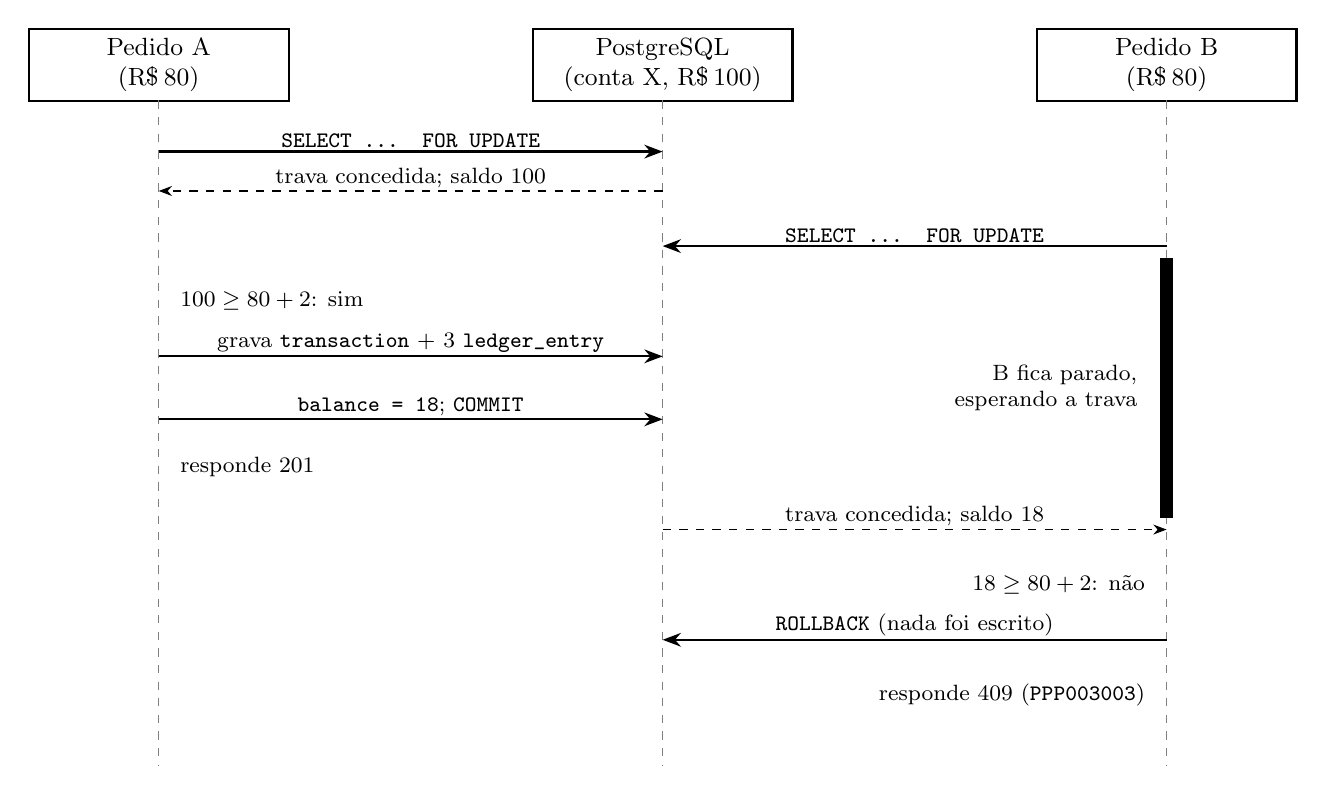
\begin{tikzpicture}[>=Stealth, font=\small,
  head/.style={draw,thick,minimum width=3.3cm,minimum height=0.9cm,align=center},
  msg/.style={->,thick},
  ret/.style={->,dashed},
  lbl/.style={font=\footnotesize,fill=white,inner sep=1pt}]
  \def\xa{0} \def\xd{6.4} \def\xb{12.8}
  % cabecas
  \node[head] at (\xa,0) {Pedido A\\(\rs 80)};
  \node[head] at (\xd,0) {PostgreSQL\\(conta X, \rs 100)};
  \node[head] at (\xb,0) {Pedido B\\(\rs 80)};
  % linhas de vida
  \foreach \x in {\xa,\xd,\xb} \draw[dashed,gray] (\x,-0.45) -- (\x,-8.9);
  % A trava
  \draw[msg] (\xa,-1.1) -- node[lbl,above] {\tb{SELECT ... FOR UPDATE}} (\xd,-1.1);
  \draw[ret] (\xd,-1.6) -- node[lbl,above] {trava concedida; saldo 100} (\xa,-1.6);
  % B tenta travar
  \draw[msg] (\xb,-2.3) -- node[lbl,above] {\tb{SELECT ... FOR UPDATE}} (\xd,-2.3);
  \fill[black] (\xb-0.08,-2.45) rectangle (\xb+0.08,-5.75);
  \node[font=\footnotesize,align=right,anchor=east] at (\xb-0.25,-4.1) {B fica parado,\\esperando a trava};
  % A decide e escreve
  \node[font=\footnotesize,anchor=west] at (\xa+0.15,-3.0) {$100 \geq 80 + 2$: sim};
  \draw[msg] (\xa,-3.7) -- node[lbl,above] {grava \tb{transaction} + 3 \tb{ledger_entry}} (\xd,-3.7);
  \draw[msg] (\xa,-4.5) -- node[lbl,above] {\tb{balance = 18}; \tb{COMMIT}} (\xd,-4.5);
  \node[font=\footnotesize,anchor=west] at (\xa+0.15,-5.1) {responde 201};
  % B recebe a trava
  \draw[ret] (\xd,-5.9) -- node[lbl,above] {trava concedida; saldo 18} (\xb,-5.9);
  \node[font=\footnotesize,anchor=east] at (\xb-0.15,-6.6) {$18 \geq 80 + 2$: não};
  \draw[msg] (\xb,-7.3) -- node[lbl,above] {\tb{ROLLBACK} (nada foi escrito)} (\xd,-7.3);
  \node[font=\footnotesize,anchor=east] at (\xb-0.15,-8.0) {responde 409 (\tb{PPP003003})};
\end{tikzpicture}
\end{center}

Sem a trava, A e B leriam \rs 100, os dois aprovariam e \rs 160 sairiam de uma conta que tinha
\rs 100. Esse é o \emph{lost update}. O \tb{CHECK (balance >= 0)} do banco ainda barraria o
segundo, mas com um 500, que é um ramo que ninguém desenhou.

\textbf{Transferência --- falha: o cliente reenvia o mesmo pedido (retentativa).} O reenvio passa
pelos passos 1 a 4. Se o original ainda está em andamento, o reenvio espera a trava no passo 4. No
passo 5 ele encontra a \tb{transaction} já gravada:
\begin{itemize}
  \item da mesma conta e com o pedido idêntico ao gravado (tipo, valor, destino e descrição,
        comparados com as colunas da \tb{transaction}), devolve 200 com o corpo original e não
        executa os passos 6 a 10, então nada é debitado de novo;
  \item de outra conta, ou com um pedido diferente (mesma chave, outro tipo ou valor, por
        exemplo), devolve 409 (\tb{PPP000004}), sem mostrar nada do pedido original.
\end{itemize}
A checagem de idempotência fica \emph{depois} da trava de propósito. Se viesse antes, um reenvio
simultâneo passaria pela checagem (o original ainda não gravou), esperaria a trava e, ao ver o saldo
já debitado, receberia um falso ``saldo insuficiente'' em vez da resposta original. O \tb{UNIQUE}
de \tb{idempotency_key} fica como rede de segurança: dois pedidos de contas diferentes com a mesma
chave, ao mesmo tempo, passam os dois pela busca, e o banco recusa o segundo (409).

\textbf{Transferência --- falha: transferências cruzadas (A $\to$ B e B $\to$ A ao mesmo
tempo).} Se cada pedido travasse primeiro a própria origem, cada um seguraria uma conta e esperaria
a outra para sempre (\emph{deadlock}). Travando sempre na ordem crescente de \tb{id}, os dois
disputam a mesma primeira trava: um passa e o outro espera.

% ---------------------------------------------------------------------
\subsubsection*{Aplicação --- caminho feliz}
\begin{enumerate}
  \item O schema exige \tb{product_key}, \tb{side = APPLY}, \tb{amount} e \tb{Idempotency-Key}.
  \item Busca o cliente e a conta do caminho, que precisa ser dele: cliente ou conta inexistente
        (ou de outro cliente), 404 (\tb{PPP001001} ou \tb{PPP002001}); conta bloqueada ou
        encerrada, 409 (\tb{PPP002005}).
  \item Busca \tb{product}; não existe, 404 (\tb{PPP005001}). O catálogo do MVP não tem produto
        inativo nem vencido. Produto com prazo (LCI) não vence como um todo: o vencimento é
        calculado no passo 11.
  \item Busca a \tb{suitability_assessment} mais recente. Confere a validade (\tb{created_at} +
        24 meses) $\geq$ hora real,
        \tb{risk_level} $\leq$ \tb{maximum_risk_level} do perfil e \tb{amount} $\geq$
        \tb{minimum_application_amount}.
  \item Busca o preço do dia: o \tb{product_price} de maior \tb{price_date} $\leq$ data de
        movimento. Ele sempre existe: o fechamento só abre um dia depois de gravar todos os preços.
  \item Trava a conta. Depois trava a \tb{position} (conta, produto), se já existir.
  \item Procura \tb{transaction} pela \tb{idempotency_key} e não encontra. (Se achar: da mesma
        conta, com uma ordem de mesmo lado, produto e valor, devolve a ordem original com 200;
        qualquer outro caso, inclusive a chave de um depósito, 409.)
  \item Confere a conta \tb{ACTIVE} e \tb{balance} $\geq$ \tb{amount}.
  \item Calcula \tb{quantity = amount / unit_price}, truncada em 8 casas, e cria a
        \tb{position} com \tb{quantity = 0} se ainda não existir.
  \item Grava \tb{transaction} \tb{INVESTMENT_APPLY} (com a \tb{idempotency_key} e o
        \tb{business_date} = data de movimento atual) e um
        \tb{ledger_entry} \tb{DEBIT}, e atualiza \tb{balance}.
  \item Grava \tb{investment_order} com \tb{transaction_id}, \tb{product_id}, \tb{quantity},
        \tb{unit_price} e \tb{acquisition_cost_amount} (= \tb{amount}). Se o produto tem prazo,
        grava também \tb{maturity_date} = data de movimento + \tb{term_months} (RN-ORD-17).
  \item Soma \tb{quantity} e \tb{amount} em \tb{position.quantity} e
        \tb{position.acquisition_cost_amount}.
  \item \tb{commit}; 201 com \tb{order_key}, \tb{quantity} e \tb{unit_price}.
\end{enumerate}

A ordem das travas é sempre \emph{conta, depois posição}. Como cada cliente tem uma só conta
aberta, a trava da conta enfileira todas as ordens daquele cliente. Por isso a posição pode ser
criada no passo 6 sem risco de duas ordens simultâneas tentarem criá-la.

\textbf{Aplicação --- falha: produto acima do perfil (a mais provável).} O passo 4 recusa antes de
qualquer trava ou escrita. O cliente recebe 422 (\tb{PPP007003}). Perfil vencido ou inexistente
recusa no mesmo passo, com 409 (\tb{PPP004004} / \tb{PPP004005}).

\textbf{Aplicação --- falha: exceção entre os passos 10 e 12 (a mais cara).} O débito já está na
sessão, mas a ordem ou a posição não foram gravadas. O \tb{rollback} desfaz débito, lançamento e
ordem juntos, e o cliente recebe 500 com o saldo intacto. É isso que garante que \emph{dinheiro
nunca sai da conta sem virar posição}.

% ---------------------------------------------------------------------
\subsubsection*{Resgate --- o que muda em relação à aplicação}
\begin{itemize}
  \item \textbf{Sem checagem de perfil no passo 4.} O cliente sempre pode tirar o dinheiro, mesmo
        com perfil vencido. No lugar dela: produto com prazo (\tb{term_months}) e data de movimento $<$
        vencimento da aplicação dá 422 (\tb{PPP007005}). Na LCI, o vencimento é o de cada aplicação
        (RN-ORD-17): vale o da aplicação mais recente ainda não liquidada. Quem devolve o
        dinheiro no vencimento é o fechamento do dia (RN-FEC-09), então o cliente não precisa
        pedir.
  \item \textbf{No passo 8,} com a posição travada, confere
        \tb{position.quantity} $\geq$ quantidade a resgatar, sendo essa quantidade
        \tb{amount / unit_price} ou toda a posição se \tb{redeem_all}.
  \item \textbf{Passos 10 a 12 invertidos:} \tb{INVESTMENT_REDEEM} com \tb{ledger_entry}
        \tb{CREDIT}. A posição perde a quantidade resgatada, e \tb{acquisition_cost_amount} cai na mesma
        proporção. Uma posição zerada fica com \tb{quantity = 0} e não é apagada.
  \item \textbf{No passo 11,} a ordem guarda em \tb{acquisition_cost_amount} o custo que saiu da posição
        (\tb{floor} proporcional; no resgate total, o \tb{acquisition_cost_amount} inteiro). A resposta
        201 traz também \tb{acquisition_cost_amount}, \tb{result_amount} = \tb{amount} $-$ \tb{acquisition_cost_amount} e
        \tb{return_bps} (RN-ORD-16).
\end{itemize}

\textbf{Encerrar conta com investimento.} O \tb{PATCH} para \tb{CLOSED} (pela rota do cliente ou
pela do banco, RN-CON-11) trava a conta e, além do
saldo zero, confere que nenhuma posição do cliente tem quantidade $> 0$; senão, 409
(\tb{PPP002004}). Como toda ordem trava a conta antes da posição, não há aplicação no meio do
encerramento.

\textbf{Resgate --- falha: valor maior que a posição.} O passo 8 recusa com a posição travada, e
nada foi escrito. O cliente recebe 409 (\tb{PPP007004}).

% ---------------------------------------------------------------------
\subsubsection*{Suitability --- caminho feliz}
\begin{enumerate}
  \item Busca o cliente pelo \tb{customer_key}.
  \item Confere sete respostas, uma por \tb{suitability_question}, cada \tb{option} pertencendo à
        sua pergunta.
  \item Soma os códigos das opções escolhidas (o código é a pontuação). Se Q3 ou Q5 tiver a
        opção 1, o perfil é \tb{CONSERVATIVE}. Se não, o perfil sai da faixa de pontos (regra
        fixa no código: 7 a 13 Conservador, 14 a 20 Moderado, 21 a 28 Arrojado).
  \item Grava a \tb{suitability_assessment} (perfil e pontuação) e as sete
        \tb{suitability_answer}. A validade (\tb{created_at} + 24 meses) e o
        \tb{forced_by_rule} (perfil fora da faixa da pontuação) são calculados, não gravados.
  \item \tb{commit}; 201 com perfil, pontuação e validade.
\end{enumerate}
A avaliação anterior não é alterada. Ela vira histórico porque o perfil vigente é sempre a
avaliação mais recente.

\textbf{Suitability --- falha: resposta faltando ou repetida.} O passo 2 recusa antes de qualquer
escrita. O cliente recebe 422 (\tb{PPP004002}).

% ---------------------------------------------------------------------
\subsubsection*{Fechamento do dia --- caminho feliz}
\begin{enumerate}
  \item O schema exige \tb{close_date} (data \tb{AAAA-MM-DD}) e nada mais.
  \item Trava a linha atual de \tb{business_day} (a de maior \tb{business_date}) com
        \tb{FOR UPDATE}.
  \item Confere \tb{close_date} = data de movimento atual, \textbf{relida depois da trava}: quem
        esperou a trava de outro fechamento ainda tem nas mãos a linha antiga (ela continua
        existindo), e só a releitura mostra a data já avançada.
  \item Calcula o próximo dia útil (sexta $\to$ segunda).
  \item Pergunta lá fora, para o novo dia: a cota do fundo (administradora), o preço dos três
        títulos (Tesouro), o CDI e a Selic (Banco Central). Cada chamada tem timeout de 5 s.
  \item Confere cada resposta: data igual à pedida, preço e taxa $> 0$, todos os produtos com
        \tb{price_source_code} presentes.
  \item Calcula CDB e LCI: preço anterior $\times (1 + c \times$ \tb{cdi_percentage_bps}$/10000)$,
        com $c = (1 + \text{CDI do dia que fecha})^{1/252} - 1$, lido de \tb{reference_rate}
        (o CDI do novo dia, que acabou de chegar, rende o fechamento seguinte).
  \item Grava os 6 \tb{product_price} e as 2 \tb{reference_rate}.
  \item \textbf{Grava a provisão do dia que fecha} (RN-REC-05 a 07): soma os saldos das contas de
        cliente, as cotas do fundo (ao preço do dia que fecha) e o custo em CDB e LCI --- a foto do
        fim do dia, antes de a liquidação mexer nos saldos --- e grava uma linha em
        \tb{revenue_accrual} com as bases, \tb{calendar_days} (até o novo dia; 3 numa sexta) e os
        valores (base $\times$ taxa do dia $\times$ dias $/ 365$, truncados).
  \item Grava o novo \tb{business_day}, antes da liquidação: as transações dela são do dia novo.
  \item \textbf{Liquida o que venceu} (RN-FEC-09): busca as aplicações com \tb{maturity_date}
        $\leq$ novo dia que nenhuma ordem aponta em \tb{matured_investment_order_id}, em ordem crescente de
        conta. Para cada uma, trava a conta e depois a posição e grava o resgate da quantidade
        inteira ao preço do novo dia: \tb{transaction} \tb{INVESTMENT_REDEEM} \textbf{sem chave
        de idempotência} (não há pedido de cliente para repetir), com \tb{business_date} = novo
        dia (o dinheiro volta antes de ele abrir), com \tb{ledger_entry}
        \tb{CREDIT} (mesmo com a conta bloqueada), \tb{investment_order} ligada a ela com
        \tb{matured_investment_order_id} = a aplicação (o \tb{UNIQUE} impede pagar duas vezes) e a posição
        reduzida.
  \item \tb{commit}; 201 com a nova data, os preços e as taxas.
\end{enumerate}

A trava da data faz dois fechamentos simultâneos virarem uma fila: o segundo encontra a data já
avançada no passo 3 e recebe 409. Os passos 5 a 7 só leem; toda escrita fica nos passos 8 a 11.
As operações de dinheiro não travam a data de movimento: uma que começou antes do fechamento e
termina depois da foto do passo 9 fica com o dia que fechou, mas fora da provisão dele (entra na do
dia seguinte). É a limitação conhecida do Módulo 8 de \tb{regras_de_negocio.tex}: alguns centavos de
estimativa, nunca dinheiro.
A liquidação trava contas e posições na mesma ordem das ordens do cliente (conta, depois
posição), então uma aplicação no mesmo instante espera em vez de causar \emph{deadlock}.

\textbf{Fechamento --- falha: erro no meio da liquidação (a mais cara).} Preços já gravados e uma
aplicação já paga, mas a próxima falha. Como tudo está no mesmo \tb{commit}, o \tb{rollback}
desfaz preços, taxas e créditos juntos: a data não anda e ninguém recebe pela metade. Chamar de
novo refaz o dia inteiro. Uma aplicação nunca é paga duas vezes: depois de paga, já existe a ordem
que aponta para ela, e o \tb{UNIQUE} de \tb{matured_investment_order_id} barraria a segunda.

\textbf{Fechamento --- falha: serviço externo fora do ar (a mais provável).} O passo 5 recebe
erro, timeout ou conexão derrubada. O banco devolve 502 (\tb{PPP005006}). Nada foi escrito: a data
de movimento continua a mesma e o preço do dia continua o último publicado (RN-PRO-04). Basta
chamar de novo quando o serviço voltar.

\textbf{Fechamento --- falha: resposta sem sentido.} O passo 6 recusa (por exemplo, cota $= 0$ ou
título faltando) com 502 (\tb{PPP005007}), também sem escrever nada. Gravar um preço errado seria
pior do que não ter preço novo: preço publicado não se reescreve (R4).

\textbf{Fechamento --- falha: clique duplo.} O segundo pedido com o mesmo \tb{close_date} espera a
trava do primeiro, encontra a data já avançada e recebe 409 (\tb{PPP000006}). Fecha-se um dia só.

% ---------------------------------------------------------------------
\bigskip
\hrule
\medskip
\textbf{Principal desafio}

\textbf{Qual é:} mover dinheiro entre contas, e entre conta e investimento, sem criar,
duplicar ou sumir com um centavo.

\textbf{Por que é difícil:} cada operação são de três a cinco escritas em tabelas diferentes. A
solução óbvia (ler o saldo, checar, escrever) quebra em três cenários. Com dois pedidos
simultâneos, os dois leem o mesmo saldo (\rs 160 saem de \rs 100). Com o cliente reenviando após um
timeout, a transferência sai duas vezes. Com uma falha no meio, o débito é gravado sem a posição.

\textbf{Como o desenho resolve:}
\begin{itemize}
  \item Uma transação de banco por operação, com \tb{commit} só na última linha: tudo ou nada.
  \item \tb{SELECT ... FOR UPDATE} nas linhas lidas para decidir, sempre na mesma ordem: contas
        por \tb{id} crescente, depois posição.
  \item Idempotência checada \emph{sob a trava}, comparando o pedido com as colunas já gravadas,
        com o \tb{UNIQUE} de \tb{idempotency_key} (única no banco inteiro) como rede de segurança.
  \item A tarifa entra na conta do banco: todo débito tem o seu crédito, e a soma de todos os
        saldos só muda com depósito, saque, aplicação e resgate.
  \item O invariante \tb{account.balance} $= \Sigma$ créditos $- \Sigma$ débitos de
        \tb{ledger_entry}, verificado por teste depois de cada cenário acima.
\end{itemize}
\hrule
% ========================= FIM DA SECAO ==============================

\end{document}
